% !TEX TS-program = pdflatex
% !TEX encoding = UTF-8 Unicode

\documentclass[12pt]{article}

\usepackage[utf8]{inputenc} 

\usepackage{geometry}
\geometry{a4paper} 
\geometry{margin=0.25in} 
\geometry{portrait}

\usepackage{amsmath}
\usepackage{physics}
\usepackage{tikz} 

\title{tikz figures}
\author{vijayabhaskar badireddi}
%\date{} 

\begin{document}
\section*{figures}

\subsection*{inclined plane}

\begin{center}
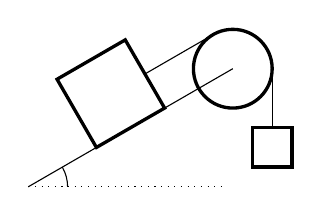
\begin{tikzpicture}[scale=0.5]

\draw [dotted] (0,0) -- (5,0) ;
\draw (0,0) -- ++(30:6) ;
\draw (1,0) arc [start angle=0,end angle=30,radius=1] ;
\draw [very thick] (30:6) circle [radius=1];
\draw (30:6) ++(0:1) -- ++(-90:1.5) ;
\draw [very thick] (30:6) ++(0:1) ++(-90:1.5) ++(-0.5,-1) rectangle ++(1,1) ;
\draw [very thick,rotate=30] (0:2) rectangle ++(2,2);
\draw (30:4) ++(120:1) -- ++(30:2) ; 

\end{tikzpicture}
\end{center}

\subsection*{pulley system 1}

\begin{center}
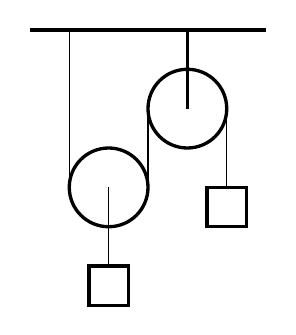
\begin{tikzpicture}[scale=0.5]

\draw [ultra thick] (0,0) -- (6,0) ;
\draw [very thick] (2,-4) circle [radius=1] ;
\draw [very thick] (4,-2) circle [radius=1] ;
\draw (1,0) -- (1,-4) (3,-4) -- (3,-2) (5,-2) -- (5,-4) ;
\draw (2,-4) -- (2,-6) ; 
\draw [very thick] (4,0) -- (4,-2) ;
\draw [very thick] (2,-6) ++(-0.5,-1) rectangle ++(1,1) ;
\draw [very thick] (5,-4) ++(-0.5,-1) rectangle ++(1,1) ;
\end{tikzpicture}
\end{center}

\subsection*{pulley system 2}

\begin{center}
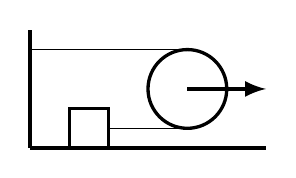
\begin{tikzpicture}[scale=0.5]

\draw [ultra thick] (0,0) -- (6,0) ;
\draw [ultra thick] (0,0) -- (0,3) ;
\draw [very thick] (4,1.5) circle [radius=1] ;
\draw (0,2.5) -- (4,2.5) ;
\draw (2,0.5) -- (4,0.5) ;
\draw [very thick] (1,0) rectangle ++(1,1);
\draw [ultra thick,-{latex}] (4,1.5) -- (6,1.5) ;
\end{tikzpicture}
\end{center}

\subsection*{pulley system 3}

\begin{center}
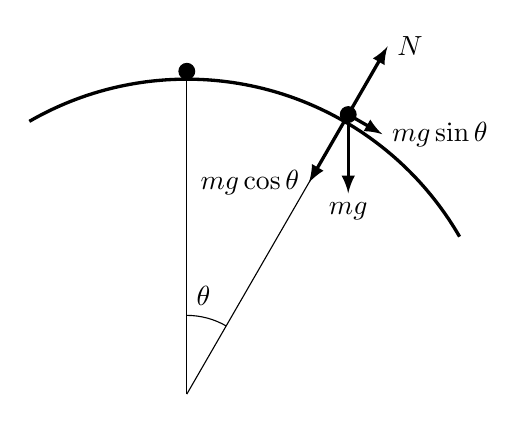
\begin{tikzpicture}[scale=1]

\draw [very thick] (0,4) arc [start angle=90, end angle= 30, radius = 4] ;
\draw [very thick] (0,4) arc [start angle=90, end angle= 120, radius = 4] ;
\draw (0,0) -- (0,4) ;
\draw [fill] (0,4.1) circle [radius=0.1] ; 
\draw [fill] (60:4.1) circle [radius=0.1] ;
\draw (0,0) -- (60:4) ;
\draw (0,1) arc [start angle =90, end angle=60,radius=1] ;
\draw (0,1) node [anchor=south west] {$\theta$} ;
\draw [very thick,-{latex}] (60:4.1) -- ++(0,-1) ;
\draw (60:4.1) ++(0,-1) node [anchor=north] {$mg$} ;
\draw [very thick,-{latex}] (60:4.1) -- ++(-120:1) ;
\draw (60:4.1) ++(-120:1) node [anchor=east] {$mg\cos\theta$} ;
\draw [very thick,-{latex}] (60:4.1) -- ++(60:1) ;
\draw (60:4.1) ++(-30:0.5) node [anchor=west] {$mg\sin\theta$} ;
\draw [very thick,-{latex}] (60:4.1) -- ++(-30:0.5) ;
\draw (60:4.1) ++(60:1) node [anchor=west] {$N$} ;

\end{tikzpicture}
\end{center}


\subsection*{hanging string}

\begin{center}
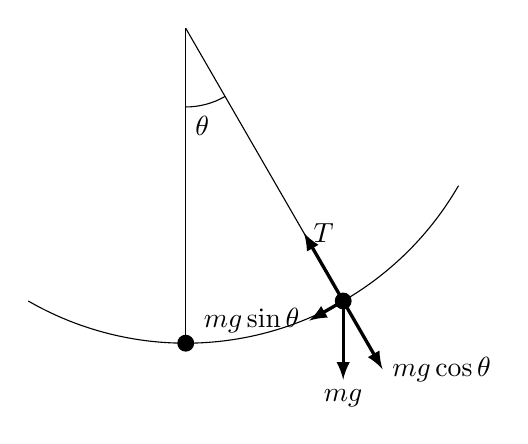
\begin{tikzpicture}

\draw (0,-4) arc [start angle=-90, end angle= -30, radius = 4] ;
\draw (0,-4) arc [start angle=-90, end angle= -120, radius = 4] ;
\draw (0,0) -- (0,-4) ;
\draw [fill] (0,-4) circle [radius=0.1] ; 
\draw [fill] (-60:4) circle [radius=0.1] ;
\draw (0,0) -- (-60:4) ;
\draw (0,-1) arc [start angle =-90, end angle=-60,radius=1] ;
\draw (0,-1) node [anchor=north west] {$\theta$} ;
\draw [very thick,-{latex}] (-60:4) -- ++(0,-1) ;
\draw (-60:4) ++(0,-1) node [anchor=north] {$mg$} ;
\draw [very thick,-{latex}] (-60:4) -- ++(-150:0.5) ;
\draw (-60:4) ++(-150:0.5) node [anchor=east] {$mg\sin\theta$} ;
\draw [very thick,-{latex}] (-60:4) -- ++(-60:1) ;
\draw (-60:4) ++(-60:1) node [anchor=west] {$mg\cos\theta$} ;
\draw [very thick,-{latex}] (-60:4) -- ++(120:1) ;
\draw (-60:4) ++(120:1) node [anchor=west] {$T$} ;

\end{tikzpicture}
\end{center}

\end{document}
